\documentclass[twoside,colorback,accentcolor=tud4c,11pt]{tudreport}
\usepackage{ngerman}
\usepackage[utf8]{inputenc} 
\usepackage[T1]{fontenc}
\usepackage{siunitx}
\usepackage{hyperref}
\usepackage{units}
\usepackage{upgreek}
\usepackage{biblatex}
\usepackage{graphicx}
\usepackage{float}
\usepackage{subfigure}
\usepackage[figure]{hypcap}
\usepackage{isotope}


\title{Versuch 4.3: Kühlen und Fangen von Rubidium-Atomen in einer MOT}
\subtitle{	\begin{tabular}{p{8cm}ll}
Dominik Pfeiffer   &   Jonas Fischer \\ Matrikelnummer: 2913632  &   Matrikelnummer: mnr       \\ email: \textaccent{ dominik@diepfeiffers.de} & email: \textaccent{email}  
			\end{tabular} }
\subsubtitle{ \\Versuchsbetreuung : Dominik Schäffner \\ Datum der Durchführung: 26.06.2017 \\ Abgabetermin:17.07.2017    }
\institution{Praktikum für Fortgeschrittene}
\sponsor{Hiermit erklären wir, dass wir die vorliegende Arbeit bzw. Leistung eigenständig, ohne fremde Hilfe und nur unter Verwendung der angegebenen Hilfsmittel angefertigt haben. Alle übernommenen Textstellen aus der Literatur beziehungsweise dem Internet sind als solche kenntlich gemacht. Diese Arbeit hat in gleicher oder ähnlicher Form noch keiner Prüfungsbehörde vorgelegen. \\\\ 
\begin{tabular}{lp{2em}lp{2em}l}
 \hspace{4cm}   && \hspace{4cm}  && \hspace{4cm}
 \\\cline{1-1}\cline{3-3}\cline{5-5}
 Ort, Datum     && Dominik Pfeiffer && Jonas Fischer
\end{tabular}  }


\dedication{}
\lowertitleback{}
\listfiles
    
\begin{document}

\maketitle 

\tableofcontents


\chapter{Einleitung und Ziel des Versuchs}
Ziel dieses Versuches ist es schrittweise eine magnetooptische Falle (MOT) aufzubauen, $\isotope[85]{Rb}$-Atome in dieser zu fangen und die Temperatur in verschiedenen Phasen der MOT zu bestimmen. Hierfür wird zunächst das zum Kühlen verwendete Lasersystem stabilisiert, dann die Ladephase der MOT überprüft und schließlich die zur Temperaturbestimmung notwendigen Messungen durchgeführt.

\chapter{Physikalische Grundlagen}
Zunächst sollen der Aufbau und dessen wichtigste Komponenten, sowie die Theorie hinter der Laserkühlung bis in den unteren Mikrokelvinbereich und das räumliche Fangen in der Falle näher betrachtet werden.
\section{Aufbau und wichtige Komponenten}
Zunächst betrachten wir den Versuchsaufbau, der sich im wesentlichen in drei Bereiche aufteilen lässt. Zunächst ist für die Datenaufnahme ein PC mit angeschlossenem digitalen Oszilloskop und einem zusätzlichen Monitor für die Live-Darstellung der Bilder der CCD-Kamera vorhanden. Des Weiteren ist die komplette Steuerungstechnik mit allen wichtigen Komponenten zur Steuerung der Laser, Magnetspulen und Kameras in einem Elektronik-Rack untergebracht. Darunter auch die drei analogen Oszilloskope, die zur Laserstabilisierung benötigt werden. Den dritten Bereich bildet der optische Aufbau, welcher komplett auf einem optischen, möglichst schwingungsarm gelagerten Tisch montiert ist, siehe Abbildung \ref{aufb}:
\begin{figure}[H]
\centering
   	\begin{minipage}[b]{0.85\textwidth}
   	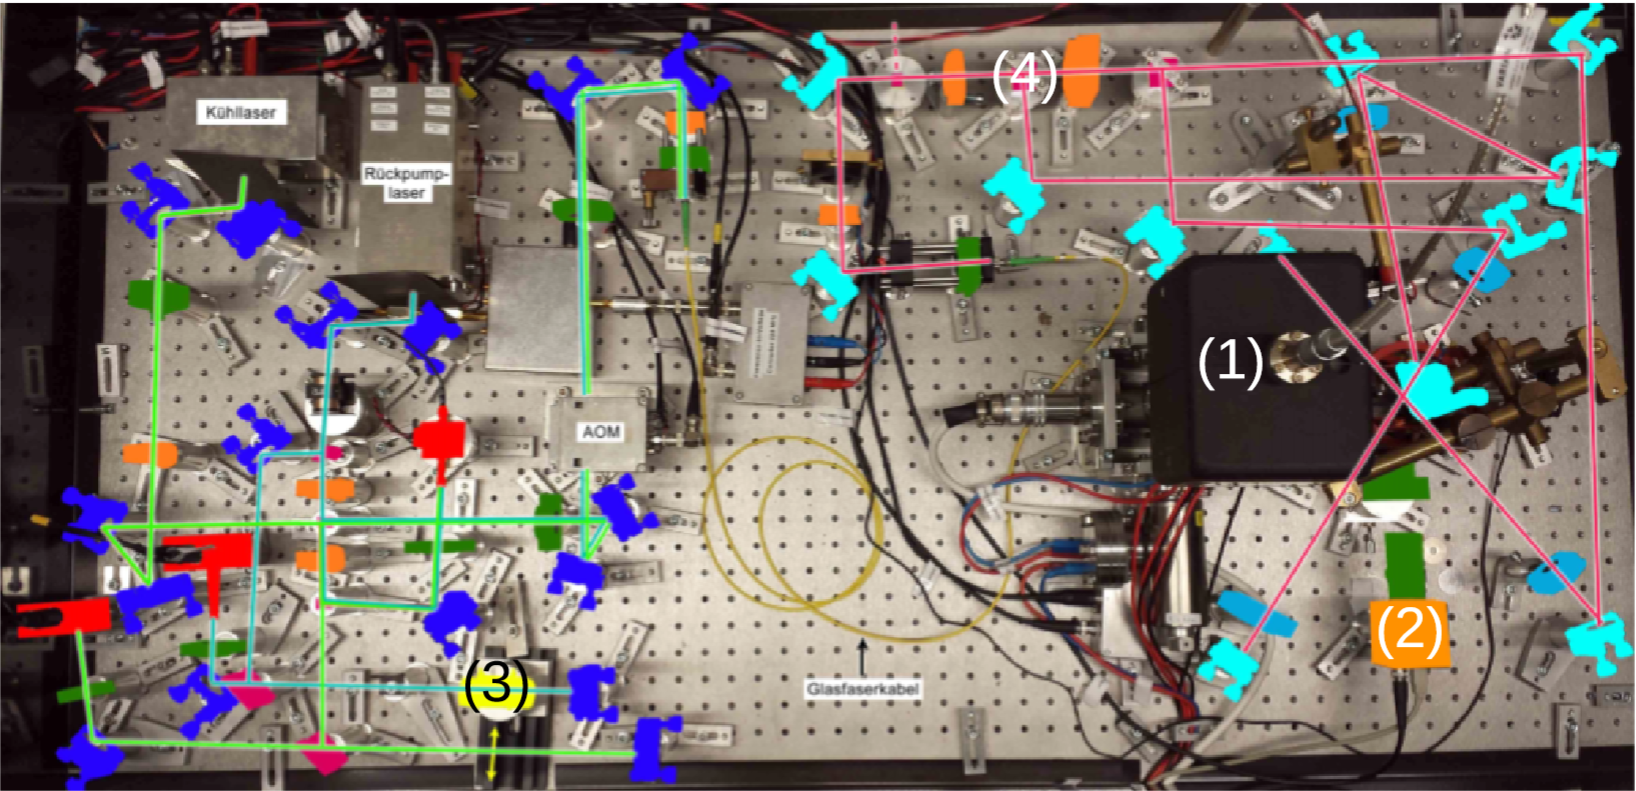
\includegraphics[width=\textwidth]{graphics/aufbau2.png}\
   	\end{minipage}
\caption{Bild von oben auf den optischen Tisch mit dem Aufbau, sowie den eingezeichneten Strahlengängen \cite{anl}}\label{aufb}	
\end{figure}
Folgend sollen die wichtigsten Komponenten des optischen Aufbaus und ihre Funktion kurz erläutert werden. Dabei wird Bezug auf die obige Abbildung genommen, in der einige Komponenten bereits eine Beschriftung tragen, andere sind farblich und/oder mit einer Nummer gekennzeichnet.
\subsection{Akusto-Optischer-Modulator (AOM)}
Der AOM ist im Aufbau in der Mitte zu sehen und trägt ebendiese Aufschrift. Dieses Bauteil besteht aus einem Kristall, einem Ultraschall-Piezoelement und einem Dämpfer. Durch das Piezoelement wird eine Ultraschallwelle in den Kristall der Frequenz $f_{AOM}=96\,\si{MHz}$ eingestrahlt, welche am anderen Ende des Kristalls vom Dämpfer absorbiert wird, wodurch das Entstehen stehender Wellen verhindert wird. Wird der Laser in den AOM eingestrahlt, sieht er aufgrund der durch die Schallwelle im Kristall verursachte Dichte- und damit Brechungsindex-Schwankung ein sich bewegendes optisches Gitter. In der ersten Beugungsordnung dieses Gitters wird die um die Frequenz des AOMs blauverschobene Laserstrahlung ausgestrahlt. Im Versuch dient der AOM hauptsächlich als Schalter, um den Laserstrahl getiehlt an-/ausschalten zu können.
\subsection{$\frac{\lambda}{2}$-/ $\frac{\lambda}{4}$-Verzögerungsplatten}
Verzögerungsplatten tragen ihre Funktion bereits im Namen. Sie bestehen aus s.g. doppelbrechenden Materialien, welche die Eigenschaft haben, verschiedenen Brechungsindices für verschieden polarisierte elektromagnetische Wellen zu haben. Damit lässt sich mit einer $\frac{\lambda}{2}$-Platte die Polarisation einer linear polarisierten Welle drehen und mit einer $\frac{\lambda}{4}$-Platte aus linearem zirkular polarisiertes Licht gewinnen. Im Versuchaufbau werden die $\frac{\lambda}{2}$-Platten (orange) benötigt um eine effiziente Teilung des Laserlichtes an den Strahlteilern zu gewährleisten und die $\frac{\lambda}{4}$-Platten (hellblau) um den Laserstrahl für die MOT zirkular zu polarisieren. Wieso dies nötig ist, wird im Kapitel zur Theorie der MOT \ref{theorie} näher erörtert.
\subsection{Polarisationsstrahlteilerwürfel (PST)}
Dieses Bauteil besteht aus einem optisch isotropen Glaswürfel ((4) siehe \ref{aufb}), in dessen Hauptdiagonale Dünnschicht-Polarisatoren eingebracht wurden. Dabei ist der Würfel als ganzes so gefertigt, dass sich die reflektierten senkrecht-polarisierten (s-pol.) Teile des eintreffenden Laserstrahles konstruktiv überlagern, während die parallel-polarisierten (p-pol.) Teile destruktiv interferieren. Der Einfallswinkel des Lichtes wird zudem als der Brewster-Winkel gewählt, wodurch keine s-pol. Teile des Strahles transmittiert werden. Durch dieses Bauteil lässt sich ein linear-polarisierter Laserstrahl in seinen s-pol. und p-pol. Teil aufspalten, da die s-Teile reflektiert und die p-Teile transmittiert werden.
\subsection{Photodiode}
In diesem Aufbau kommen an drei Stellen Photodioden zum Einsatz (Rot markiert). Es handelt sich bei einer Photodiode um ein Halbleiterbauteil mit einem p-/ und einem n-dotierten Teil. Dotierung heißt, dass das Trägermaterial gewollt mit Fremdatomen mit einem Hüllenelektron weniger (p-Dotierung) bzw. einem Hüllenelektron mehr (n-Dotierung) verunreinigt. Durch den Kontakt von p- und n-dotierten Halbleiter bildet sich eine Sperrschicht aus, welche durch Anlegen einer äußeren Spannung vergrößert (Sperrrichtung) oder verkleinert (Durchlassrichtung) werden kann. Im Versuch wird eine s.g. pin-Diode verwendet, welche zwischen den dotieren Teilen einen sehr schwach oder nicht dotierten Teil (i-Teil) besitzt. Trifft ein Photon durch die Öffnung auf die Diode, so kommt es bei der Absorption des Photons zur Bildung von Elektron-Loch-Paaren, welche durch das elektrische Feld der Sperrschicht voneinander getrennt werden und als messbarer Strom über Kathode und Anode der Diode ab. Im Versuch kommen die Dioden zum einen bei der Spektroskopie des Rückpumplasers zum Einsatz, als auch bei der Ofsetstabilisierung des Kühllasers.
\subsection{Ion-Getter-Pumpe (IGP)}
Die IGP ((1) siehe \ref{aufb}) ist für das Aufrechterhalten des Vakuums in der MOT zuständig und aufgrund dessen permanent in Betrieb. Sie funktioniert nicht wie eine herkömmliche Pumpe mit beweglichen Teilen und einer Auslassöffnung, sondern elektronisch. Im Inneren befinden sich waagerechte Anodenröhrchen sowie ein Kathodenblech (Getter) zwischen denen eine Spannung von $U_{IGP}\approx 7\,\si{kV}$ anliegt. Des Weiteren befinden sich am Rand Magnete, welche für ein statisches, parallel zu den Röhrchen verlaufendes Magnetfeld sorgen. Durch die Hochspannung bilden sich Elektronenwolken und die freien Elektronen werden durch das Magnetfeld auf eine Spiralbahn gezwungen (Lorentz-Kraft $\vec{F_{L}}=q \vec{v} x \vec{B}$). Stoßen diese Elektronen mit Atomen des durch die Pumpe strömenden Restgases, werden diese ionisiert, durch das elektrische Feld beschleunigt und durch den Aufprall auf dem Kathodenblech in diesem gefangen. Beim Aufprall der ionisierten Restgasatome kommt es zur dazu, dass Kathodenmaterial aufgewirbelt wird und so stets neues Material an der Oberfläche vorhanden ist um weiter Restgasatome zu fangen.
\subsection{Rubidiumgaszelle}
Hierbei handelt es sich um eine elektrisch geheizte Zelle mit $\isotope[85]{Rb}$ im inneren, welche für die dopplerfreie Sättigungsspektroskopie und damit die Stabilisierung des Rückpumplasers verwendet wird. In Abbildung \ref{aufb} ist sie mit (3) gekennzeichnet
\subsection{CCD-Kamera}
Die Kamera (2) wird dazu verwendet, um ein stetiges Live-Bild der MOT auf einem extra Monitor darstellen zu können. Dies ist notwendig um im Laufe des Versuches während der Messungen die korrekte Funktion der MOT überprüfen zu können und Notfalls die Messung zu stoppen um eventuelle Fehler zu korrigieren.
\section{Theorie zur Laserstabilisierung}
\subsection{Dopplerfreie Sättigungsspektroskopie}
\subsection{Ofsetlock}
\section{Theorie zur MOT}\label{theorie} 	
\chapter{Versuchsdurchführung und Auswertung}
\section{Stabilisierung des Lasersystems}
\section{Ladephase der MOT}
\section{Temperaturbestimmung in der MOT}
\subsection{Temperatur der MOT}
\subsection{Temperatur in der optischen Melasse}
\chapter{Diskussion}
\chapter{Messdaten}


\chapter{Anhang}





		

\renewcommand{\bibname}{Literaturverzeichnis}
\begin{thebibliography}{Bak89}
\bibitem {anl} Anleitung zum Versuch 4.3: MOT, (Stand 26.06.2017)


\end{thebibliography} 	



\end{document} 